\documentclass[12pt,letterpaper,pdftex]{article}

\usepackage[authoryear]{natbib}
\usepackage{times} 
\usepackage{amsmath,amsfonts}
\usepackage{graphicx}
\usepackage{setspace}
\usepackage{indentfirst}
\usepackage{color}

% revise margins
\setlength{\headheight}{0.0in}
\setlength{\headsep}{0.0in}
\setlength{\topmargin}{0.0in}
\setlength{\textheight}{8.9in}
\setlength{\footskip}{0.4in}
\setlength{\oddsidemargin}{0.1in}
\setlength{\evensidemargin}{0.1in}
\setlength{\textwidth}{6.3in}

\setlength{\rightskip}{0pt plus 1fil} % makes ragged right

% bibliography format
\usepackage[authoryear]{natbib}
\bibpunct{(}{)}{;}{a}{}{,}

% environment for Figure legends
\newenvironment{hanging}
{\begin{list}{}
        {\setlength{\labelwidth}{0in}
         \setlength{\leftmargin}{1em}
         \setlength{\itemindent}{-1em}
        }
}
{\end{list}}

\begin{document}
\setstretch{2.0}

\vspace*{1in}

\begin{center}
\textbf{\Large Haplotype probabilities in
advanced intercross populations}

\bigskip \bigskip \bigskip \bigskip 
 
{\large Karl W. Broman$^1$

\bigskip \bigskip

Department of Biostatistics and Medical Informatics, \\
University of Wisconsin--Madison, Madison, Wisconsin 53706 }
\end{center}


\vfill

\hfill 
{\footnotesize 28 October 2011}

\newpage

\noindent \textbf{Running head:} AIL haplotype probabilities


\bigskip \bigskip \bigskip

\noindent \textbf{Key words:} advanced intercross lines, heterogeneous
stock, diversity outcross, map expansion, Collaborative Cross



\bigskip \bigskip \bigskip

\noindent \textbf{$^1$Corresponding author:}

\begin{tabular}{lll}
 \\
 \hspace{1cm} & \multicolumn{2}{l}{Karl W Broman} \\
 & \multicolumn{2}{l}{Department of Biostatistics and Medical Informatics} \\
 & \multicolumn{2}{l}{University of Wisconsin--Madison} \\
 & \multicolumn{2}{l}{1300 University Ave, Rm 4710 MSC} \\
 & \multicolumn{2}{l}{Madison, WI 53706} \\
 \\
 & Phone: & 608--262--4633 \\
 & Fax: & 608--265--7916 \\
 & Email: & \verb|kbroman@biostat.wisc.edu|
\end{tabular}



\clearpage
\centerline{ABSTRACT} 
  
Advanced intercross populations have the advantage
of greater precision of genetic mapping, due to the
accumulation of recombination events across the multiple generations.  Related designs include
heterogeneous stock and the diversity outcross population.
We derive the two-locus haplotype probabilities on the autosome and X
chromosome with these designs.





\newpage
% Note: selective genotyping 'Note' was 7 pages of text + 3 figs
%       and ended up being 4 published pages.

Advanced intercross populations, in which multiple inbred strains are
mated at random for many generations, have the advantage
of greater precision of genetic mapping, due to the
accumulation of recombination events across the multiple generations.
The most commonly used form, which
begins with two inbred strains, was formally introduced by
\citet{Darvasi1995} and called advanced intercross lines (AIL).  A
closely related design is that of heterogeneous stock \citep[HS;
see][]{Mott2000}, in which eight inbred strains are randomly mated
for many generations.  \citet{Svenson2012} developed
the diversity outcross population (DO), which was formed with
progenitors that were partially inbred individuals drawn from intermediate
generations in the development of the Collaborative Cross
\citep[so-called pre-CC mice; see][]{Aylor2011}.

The mapping of quantitative trait loci (QTL) in such populations,
whether by interval mapping \citep{Lander1989} or Haley-Knott
regression \citep{Haley1992}, generally requires conditional genotype
probabilities at putative QTL, given the available marker genotype
data. Such probabilities are often calculated using a hidden
Markov model \citep[HMM; see][App. D]{Broman2009}.  An HMM for this purpose
formally requires the calculation of two-locus diplotype probabilities, though
if the populations are formed with a large number of mating pairs, the
two haplotypes within an individual are independent, and so it is
sufficient to calculate two-locus haplotype probabilities.

\citet{Darvasi1995} derived the two-locus haplotype probabilities for
the autosome in
AIL.  I am not aware of any work considering the X chromosome.  In
this paper, I derive the two-locus haplotype probabilities for the
autosome and X chromosome in AIL, HS and the DO.  The calculations for
the DO rely on recent results on haplotype probabilities in pre-CC
mice \citep{Broman2012}.  Throughout, I assume an effectively
infinite set of mating pairs at each generation, no sex difference in
recombination, and no selection or mutation.

Let us first revisit the two-locus autosomal haplotype probabilities in
AIL, as they serve as a simple example of the technique used in these 
calculations 
\citep[see also][Ch. 3]{Bulmer1980}. Let $p_s$ denote the frequency of
the $AA$ haplotype at generation $\text{F}_s$.  Then $p_1 = \frac{1}{2}$ and
we have the recurrence relation
\begin{equation}
p_{s+1} = \textstyle{ (1-r) p_s + r \cdot \frac{1}{2} \cdot
  \frac{1}{2} }
\label{eqn:ailA}
\end{equation}
where $r$ is the recombination fraction (in one meiosis) between the
two loci.  Equation (\ref{eqn:ailA}) is derived by noting that 
an $AA$ haplotype drawn from generation $\text{F}_{s+1}$
is either an intact $AA$ haplotype at generation $\text{F}_s$,
transmitted without recombination, or it is a recombinant haplotype
bringing two independent $A$ alleles together.
Note that the frequency of the $A$ allele is $\frac{1}{2}$ at every
generation.  

The solution of this recurrence relation \citep[see][]{Graham1994} is, for $s \ge 2$,
\begin{equation}
p_s  = \textstyle{ \frac{1}{4}\left[1 + (1-2r)(1-r)^{s-2}\right] }.
\end{equation}
The frequency of recombinant haplotypes at generation $\text{F}_s$ is
$1-2p_s$.

For the X chromosome in AIL, I will first consider a balanced case, begun
with equal proportions of $\text{F}_1$ individuals from reciprocal
crosses, $A \times B$ and $B \times A$, so that 
the $\text{F}_1$ males are equally likely to be hemizygous $A$ or
$B$.  Let $m_s$ and $f_s$ denote the frequency of the AA haplotype in
males and females, respectively, at generation $\text{F}_s$.  Then $m_1 = f_1 = \frac{1}{2}$ and we have
\begin{equation} \begin{split}
m_{s+1} & = \textstyle{ (1-r)f_s + \frac{r}{4} } \\[6pt]
f_{s+1} & = \textstyle{ \left(\frac{1}{2}\right)m_s + \left(\frac{1-r}{2}\right)
  f_s + \frac{r}{8} } 
\label{eqn:ailXbalrecur}
\end{split} \end{equation}
This recurrence relation is derived in a similar way to that for the
autosome, noting that the male haplotype was drawn from his mother,
with a chance for recombination, and a random female haplotype is
equally likely to have been drawn from her father, without recombination, or
from her mother, with the potential for recombination.  I again make
use of the fact that the frequency of the $A$ allele is $\frac{1}{2}$ in
both males and females at every generation.  The solution to this
relation is, for $s \ge 2$,
\begin{equation} \begin{split}
m_s & = \textstyle{ \frac{1}{8} \left[2 + (1-2r)(w^{s-2} + y^{s-2}) + 
\left(\frac{3 - 5r + 2r^2}{z}\right)(w^{s-2} - y^{s-2})\right] } \\[6pt]
f_s & = \textstyle{ \frac{1}{8} \left[2 + (1-2r)(w^{s-2} + y^{s-2}) + 
\left(\frac{3 - 6r + r^2}{z}\right)(w^{s-2} - y^{s-2})\right] }
\label{eqn:ailXbalsoln}
\end{split} \end{equation}
where $z = \sqrt{(1-r)(9-r)}$, $w = (1-r+z)/4$ and $y =(1-r-z)/4$.
Note that the frequencies of recombinant haplotypes in males and
females are $1-2m_s$ and $1-2f_s$, respectively, and that the overall
frequency is $1 - (2m_s + 4f_s)/3$.

Now I turn to the unbalanced case for the X chromosome, in which all
$\text{F}_1$ individuals are derived from the cross $\text{female } A
\times \text{male } B$, so that all $\text{F}_1$ males are hemizygous
$A$.  This appears to be widely used in practice
\citep[e.g.,][]{Norgard2008, Kelly2010}.  The calculations are more
difficult,  because the allele frequencies are
different in males and females and across generations.

I first calculate the single-locus allele frequencies.
Let $q_s$ be the
frequency of the $A$ allele in females at generation $\text{F}_s$.
Note that the frequency in males at $\text{F}_s$ is $q_{s-1}$.
The initial values are $q_0 = 1$ and $q_1 = \frac{1}{2}$, and we have the
recurrence relation $q_{s+1} = \frac{1}{2}q_s + \frac{1}{2}q_{s-1}$,
which comes from the fact that a random allele drawn from the female
at generation $\text{F}_{s+1}$ is equally likely to be an allele from the
female or male at generation $\text{F}_s$, and the allele in the male
at $\text{F}_s$ is a random allele from the female at $\text{F}_{s-1}$.
The solution of the recurrence relation is $q_s = \frac{2}{3} +
(\frac{1}{3})(-\frac{1}{2})^s$, for $s \ge 0$. 

I now turn to the two-locus haplotype probabilities.  Let $m'_s$ and
$f'_s$ denote the frequencies of the $AA$ haplotype on the X
chromosome in males and
females at generation $\text{F}_s$ in an unbalanced AIL, and note that
$m'_1 = 1$ and $f'_1 = \frac{1}{2}$.  The haplotype probabilities
satisfy a recurrence relation similar to that in equation (\ref{eqn:ailXbalrecur}):
\begin{equation} \begin{split}
m'_{s+1} & = (1-r) f'_s + r q_{s-1} q_{s-2} \\[6pt]
f'_{s+1} & = \textstyle{ \left(\frac{1}{2}\right)m'_s + \left(\frac{1-r}{2}\right)
  f'_s + \left(\frac{r}{2}\right) q_{s-1} q_{s-2} }
\label{eqn:ailXub}
\end{split} \end{equation}

Note the distinction between equations (\ref{eqn:ailXbalrecur}) and
(\ref{eqn:ailXub}):  if a recombinant haplotype is transmitted
from the $\text{F}_s$ female, the chance that it brings two $A$
alleles together depends on the frequency of the $A$ allele in males
and females in the $\text{F}_{s-1}$ generation.  In the balanced case,
these are each $\frac{1}{2}$; in the unbalanced case, they are
different from each other and vary across generations.

I have been unable to obtain closed-form solutions for $m'_s$ and
$f'_s$.  However, the values can be quickly calculated numerically,
using equation (\ref{eqn:ailXub}).  Note that $\lim_{s \rightarrow \infty}
f'_s = \lim_{s \rightarrow \infty} m'_s = \frac{4}{9}$.

Haplotype probabilities in the DO are
calculated similarly.  The progenitors for the DO were pre-CC mice.
I assume a large number of progenitors, that they
were drawn from independent lines, and that the order of the crosses
that generated the different lines were random, giving complete
balance across the eight alleles.  

In a potential abuse of notation, I will redefine the $q$'s, $p$'s,
$m$'s and $f$'s used above.  Let $q_k$ denote the frequency of the
$AA$ haplotype at generation $\text{G}_2:\text{F}_k$ in the pre-CC;
this is $\frac{1-r}{2}$ times the haplotype probability in Table~4 of
\citet{Broman2012}.  Let $p_s$ be the probability of the $AA$
haplotype at generation $s$ of the diversity outcross.

The pre-CC progenitors of the DO were drawn from independent lines at
a variety of different generations along the course to inbreeding.
Let $\alpha_k$ denote the proportion of the pre-CC progenitors that
were at generation $\text{G}_2:\text{F}_k$, and note that a pre-CC
progenitor at generation $\text{G}_2:\text{F}_k$ will transmit the
$AA$ haplotype with frequency $q_{k+1}$ (that is, the frequency of the
$AA$ haplotype at generation $\text{G}_2:\text{F}_k$).  Thus, the
frequency of the $AA$ haplotype at the first generation of the DO is
$p_1 = \sum_k \alpha_k q_{k+1}$.

The recurrence relation for the $p_s$ is like that in equation
(\ref{eqn:ailA}): $p_{s+1} = (1-r)p_s + r/64$.  The solution is
\begin{equation}
p_s = \textstyle{ \frac{1}{64} + (1-r)^{s-1}\left(p_1 - \frac{1}{64}\right) }
\end{equation}
Note that the recombinant haplotypes are all equally likely, due to the
random order of the initial crosses, and so each has probability
$(1-8p_s)/56$.  

HS corresponds to the DO with $\alpha_1 = 1$ (that is, $k \equiv 1$), in which case $p_1 = q_2
= 7 - 24r + 24r^2 - 8r^3$.

I now turn to the X chromosome.  Let $m_s$ and $f_s$ denote the
frequency of the $AA$ haplotype on the X chromosome in males and
females in the DO at generation $s$.  Assuming random orders of
crosses to generate the pre-CC progenitors, 
\begin{equation}
f_1 = \textstyle{ \sum_k \alpha_k \left(\frac{1}{8}\right) \left[ (2-r) h_{k+1}^{AA} +
  (1-r) h_{k+1}^{CC} \right] }
\end{equation}
where $h_{k+1}^{AA}$ and $h_{k+1}^{CC}$ are the frequencies of the $AA$
and $CC$ haplotypes, respectively, on the X chromosome in females at
generation $\text{G}_1:\text{F}_{k+1}$ in the construction of four-way
RIL by sibling mating \citep[see][Table~4]{Broman2012}.  $m_1$ is
calculated in the same way.  The recurrence relations are much like
equation (\ref{eqn:ailXbalrecur}):
\begin{equation} \begin{split}
m_{s+1} & = \textstyle{ (1-r) f_s + \frac{r}{64} } \\[6pt]
f_{s+1} & = \textstyle{ \left(\frac{1}{2}\right)m_s + \left(\frac{1-r}{2}\right) f_s + \frac{r}{128} }
\end{split} \end{equation}
The solutions are the following:
\begin{equation} \begin{split}
m_s & = \textstyle{ \frac{1}{128} \left\{ 2 + \left[\frac{(64m_1 - 256f_1 + 3)(1-r)}{z}\right](y^{s-1} - w^{s-1})
 - (1-64m_1)(w^{s-1}+y^{s-1})\right\} } \\[6pt]
f_s & = \textstyle{ \frac{1}{128} \left\{ 2 + \left[\frac{-64f_1(1-r) -128m_1 + 3 - r}{z}\right](y^{s-1} - w^{s-1})
 - (1-64f_1)(w^{s-1}+y^{s-1})\right\} }
\end{split} \end{equation}
where $w$, $y$ and $z$ are as in equation (\ref{eqn:ailXbalsoln}).

Again, HS corresponds to DO with $\alpha_1 = 1$, in which case $f_1 =
(4-5r+r^2)/32$ and $m_1 = (2-3r+r^2)/16$.

In Figure~1, the probabilities of recombinant two-locus haplotypes are
displayed for the
different populations.  For the DO, I used the distribution of $k$ as
in Figure~1 of \citet{Svenson2012} and $s=5$.
For HS and AIL, I used $s=$ 10 and 12, respectively, to match the
total number of generations with recombination (the average $k$ in
\citet{Svenson2012} was 6).  Recombinant
haplotypes are more frequent on the autosome, and are more frequent in
HS than in the DO; inbreeding in the pre-CC progenitors of the DO is
accompanied by a loss of recombinants.

It is particularly interesting to consider the map expansion in these
populations, which is the frequency of recombination breakpoints on a
random chromosome.  Let $R$ denote the probability of a recombinant
haplotype; then the map expansion is $\left. \frac{dR}{dr}
\right|_{r=0}$ \citep[see][]{Teuscher2007}.  The map expansion on an
autosome in AIL is $s/2$.  For the DO, on an autosome, the map
expansion satisifies $M_s = \frac{7}{8}(s-1) + M_1$, where $M_1$ is
the weighted average (with weights $\alpha_k$) of the map expansion in
the pre-CC at generation $\text{G}_2:\text{F}_{k+1}$
\citep[see][Table~4]{Broman2012}.  For the particular progenitors detailed
in \citet[Figure~1]{Svenson2012}, this is approximately $(7s+37)/8$.  For HS, we have
$M_1 = 3$ and $M_s = \frac{7s+17}{8}$.

For the X chromosome in balanced AIL, HS and DO, the map expansion is
$\frac{2}{3}$ that of the autosome.  For the case of the X chromosome in
unbalanced AIL, in which all $\text{F}_1$ males are hemizygous $A$, I
cannot derive a closed-form solution, but taking the derivatives of
the recurrence relations in equation (\ref{eqn:ailXub}), I can derive
a simple recurrence relation for the map expansion.  (Note that the
overall map expansion on the X chromosome can be obtained as the
average of the sex-specific map expansions, with $\frac{2}{3}$ weight
given to the female, since two-thirds of the X chromosomes are in females.)
Let $M'_s$ denote the map expansion at
$\text{F}_s$, and again let $q_s$ be the frequency of the $A$ allele
in females at $\text{F}_s$.  Then we have
\begin{equation}
M'_{s+1} = \textstyle{ M'_s + \frac{4}{3}(q_s - q_{s-1} q_{s-2}) }
\end{equation}
with the initial conditions $M'_1 = 0$ and $M'_2 = \frac{2}{3}$.
While I have not been able to derive a closed-form solution for
$M'_s$, it is easily calculated numerically.  

The haplotype probabilities calculated above provide the key
quantities for developing HMMs for advanced intercross populations.
However, it should be noted that there are other approaches to
handling such data.  For example, \citet{Besnier2011} used a variance
components model to analyze outbred chicken AIL data, with
identity-by-descent (IBD) probabilities calculated using a modified
version of the method of \citet{PongWong2001}, for general pedigree
data.

The above result for HS differs from that in \citet{Mott2000} and
incorporated into the HAPPY software.  They had assumed that the map
expansion in HS was $\frac{7}{8}(s+2)$, while I show it
to be $\frac{7}{8}(s-1) + 3$.  In the first three of generations with
recombination, individuals are fully heterozygous, and so all
recombination events can be seen; in the subsequent $s-1$ generations,
there is a $1/8$ chance of homozygosity and so only $7/8$ of
recombination events can be seen.

\citet{Mott2000} further assumed that the transition probabilities
along an HS chromosome are a function of genetic distance, but that
requires knowledge of the map function.  It is more
direct to express the transition probabilities in terms of the
recombination fraction at meiosis.

The green curve in Figure~1 displays the probability of a recombinant
haplotype assumed in \cite{Mott2000} for HS with $s=10$, using 
the map function corresponding to the gamma model with the level of
crossover interference estimated for the mouse in \citet{Broman2002}.
The probability is slightly smaller than that from our calculations; at
$r=0.01$, the equation in \citet{Mott2000} gives 0.099, whereas I
obtain 0.103.

I have assumed an effectively infinite number of mating pairs at each
generation.  In practice, with a finite number of mating pairs, there
will be some inbreeding and so an increased frequency of homozygosity
and a decreased frequency of recombination.  In addition, the
individuals at the final generation will include siblings, and the
relationships among individuals might be used to improve the
genotype reconstruction.  In practice, for computational efficiency,
both the inbreeding and the relationships among individuals would
probably be ignored in the genotype reconstruction, and with dense
genotype data, there will be little loss of information.


\bigskip \bigskip \bigskip

\noindent \textbf{\sffamily Acknowledgments}
\bigskip

Jim Crow generously provided comments for improvement of
the manuscript.  
This work was supported in part by
National Institutes of Health grant GM074244.




\newpage 


\clearpage
\bibliographystyle{genetics}
\renewcommand*{\refname}{\normalsize\sffamily Literature Cited}
\bibliography{ailprob}


\newpage


\centerline{FIGURE LEGENDS}

\begin{hanging}

\item \textbf{Figure 1.}  
  Frequency of a two-locus haplotype being recombinant, as a function
  of the recombination fraction at meiosis, for the diversity outcross
  population at $s=5$ (solid curves), heterogeneous stock at $s=10$
  (dashed curves) and balanced AIL at $s=12$ (dotted curves), for the autosome
  (black), male X (blue) and female X (red).  The green dashed curve is
  the recombinant frequency for HS at $s=10$ assumed in
  \citet{Mott2000}.


\end{hanging}

\newpage


%%%%%%%%%%%%%%%%%%%%%%%%%%%%%%%%%%%%%%%%%%%%%%%%%%%%%%%%%%%%%%%%%%%%%%
% FIGURES
%%%%%%%%%%%%%%%%%%%%%%%%%%%%%%%%%%%%%%%%%%%%%%%%%%%%%%%%%%%%%%%%%%%%%%

\begin{figure}
\centering
\includegraphics[width=\textwidth]{Figs/fig1.eps}

\bigskip
\caption{Frequency of a two-locus haplotype being recombinant, as a
  function of the recombination fraction at meiosis, for the
  diversity outcross population at $s=5$ (solid curves), heterogeneous
  stock at $s=10$ (dashed curves) and balanced AIL at $s=12$ (dotted curves),
  for the autosome (black), male X (blue) and female X (red).  The
  green dashed curve is the recombinant frequency for HS at $s=10$
  assumed in \citet{Mott2000}.\label{fig:one}}
\end{figure}


\end{document}
